\section{Architecture}
\label{sec:architecture}

A criminal network analytics application requires real-time processing of heterogeneous data from multiple distributed sources.

In an widely extended criminal scenario, the amount of data is  huge, heterogeneous and generated rapidly. In order to extract valuable information from such datasets, systems must be highly scalable, provide high throughput and rapid exploration of 
%: a large number of people, criminals, devices, and sensors are connected via digital networks, and their interactions generate enormous valuable information \cite{FrameworkBigdata}. For these reasons, we are interested to an high-throughput and scalable process of analysis.
%Furthermore, application usage as a tool to support the law enforcement agencies, it requires the storage capacity of the social network in a database that can be consulted rapidly.

Considering these requirements, we propose an application that follows a \textit{data stream processing} approach. 
DSP is a computational paradigm in which the sources emit continuous data \textit{streams}, which are then processed in real-time by distributed and parallel operators.
Our application leverages \textit{Apache Flink} \cite{flink} as a DSP framework. 

Data aggregation is provided by \textit{Apache Kafka} \cite{kafka}, an high-throughput message queuing system, designed for making streaming data available to consumer. Kafka implements a \textit{publish/subscribe} mechanism for \textit{asynchronous communication} of data.

Criminal network graph is stored in \textit{Neo4j} \cite{neo4j}, that is a highly scalable, native graph database. Neo4j optimizes the storage of large graphs and provides a web-based interactive exploration of them.

In Figure~\ref{fig:topology} we represent the topology of operators implemented in Flink and their interactions with Kafka and Neo4j. Both link mining metrics are computed in parallel, scores are then filtered with a custom thresholding process and the output is the set of hidden and potential links.
 
%\begin{figure}[]
%	\centering
%	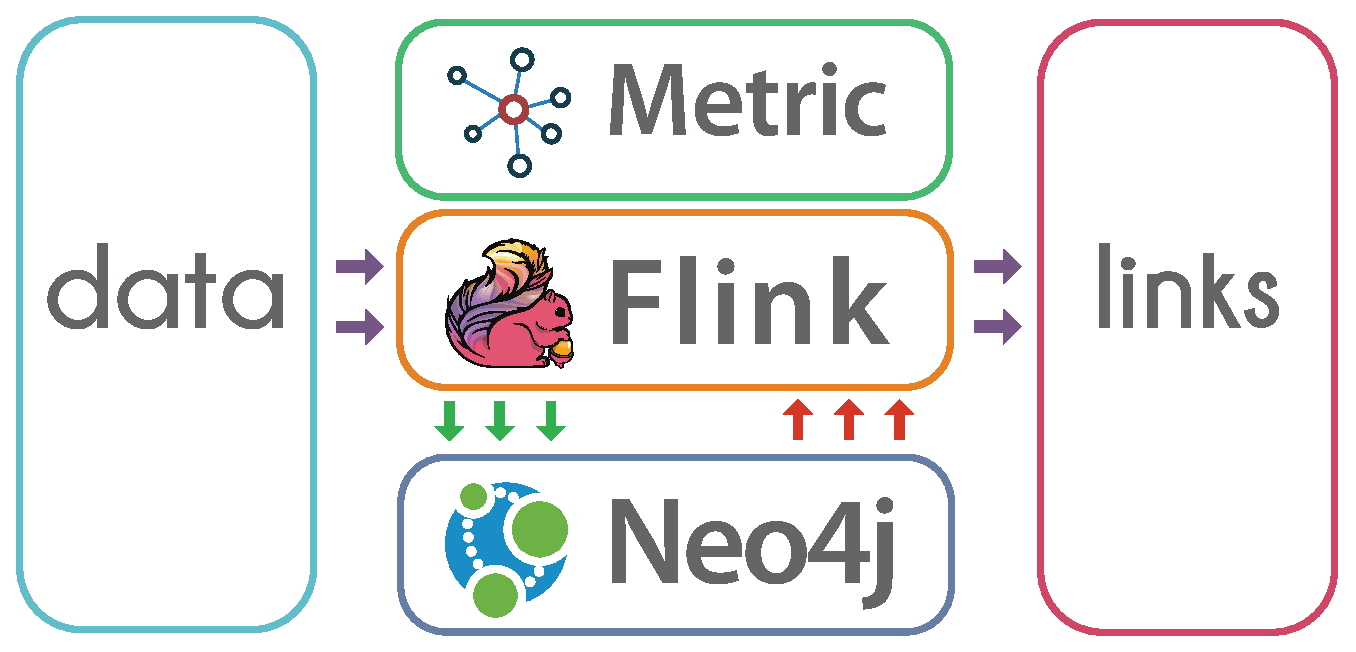
\includegraphics[width=0.48\textwidth]{fig/crimegraph-layered-architecture.eps}
%	\caption{High-level architecture.}
%	\label{fig:layered-architecture}
%\end{figure}

\begin{figure*}
\centering
\includegraphics[width=6in]{./fig/topology}
\caption{The topology of architecture.}
\label{fig:topology}
\end{figure*}

